%%%%%%%% ICML 2018 EXAMPLE LATEX SUBMISSION FILE %%%%%%%%%%%%%%%%%

\documentclass{article}

% Recommended, but optional, packages for figures and better typesetting:
\usepackage{microtype}
\usepackage{graphicx}
\usepackage{subfigure}
\usepackage{booktabs} % for professional tables

% hyperref makes hyperlinks in the resulting PDF.
% If your build breaks (sometimes temporarily if a hyperlink spans a page)
% please comment out the following usepackage line and replace
% \usepackage{icml2018} with \usepackage[nohyperref]{icml2018} above.
\usepackage{hyperref}

% Attempt to make hyperref and algorithmic work together better:
%\newcommand{\theHalgorithm}{\arabic{algorithm}}

% Use the following line for the initial blind version submitted for review:
%\usepackage[accepted]{icml2018}
\usepackage{icml2018}

%include our package here
\usepackage[colorinlistoftodos]{todonotes}
\usepackage{verbatim}
\usepackage[ruled,linesnumbered,vlined]{algorithm2e}
\usepackage{amssymb}

%defined our command here
\newcommand{\citeasnoun}[1]{\cite{#1}}
\newcommand*{\rom}[1]{\expandafter\@slowromancap\romannumeral #1@}
\makeatother
\newcommand{\E}{\mathbb{E}}
\renewcommand{\P}{\mathbb{P}}
\newcommand{\setsep}{~:~}
\newcommand{\opt}{^\star}
\newenvironment{mprog}{\begin{array}{>{\displaystyle}l>{\displaystyle}l>{\displaystyle}l}}{\end{array}}
\newcommand{\stc}{\\[1ex]  \mbox{s.t.} &}
\newcommand{\cs}{\\[1ex] & }
\newcommand{\minimize}[1]{\min_{#1} &}
\newcommand{\maximize}[1]{\max_{#1} &}
\newcommand{\tr}{^{\mathsf{T}}}
\newcommand{\one}{\mathbf{1}}
\newcommand{\Real}{\mathbb{R}}
\renewcommand{\ss}{~:~}

\newcommand{\eye}{\mathbf{I}}
\newcommand{\zero}{\mathbf{0}}

%\newcommand{\fix}[1]{}
\newcommand{\fix}[1]{{$\langle${\color{red}\sc Fix: #1}$\rangle$}}

% If accepted, instead use the following line for the camera-ready submission:
%\usepackage[accepted]{icml2018}

% The \icmltitle you define below is probably too long as a header.
% Therefore, a short form for the running title is supplied here:
\icmltitlerunning{OFVF}

\begin{document}

\twocolumn[
\icmltitle{OFVF}

% It is OKAY to include author information, even for blind
% submissions: the style file will automatically remove it for you
% unless you've provided the [accepted] option to the icml2018
% package.

% List of affiliations: The first argument should be a (short)
% identifier you will use later to specify author affiliations
% Academic affiliations should list Department, University, City, Region, Country
% Industry affiliations should list Company, City, Region, Country

% You can specify symbols, otherwise they are numbered in order.
% Ideally, you should not use this facility. Affiliations will be numbered
% in order of appearance and this is the preferred way.
\icmlsetsymbol{equal}{*}

\begin{icmlauthorlist}
\icmlauthor{Tianyi Gu}{equal,unh}
\icmlauthor{Reazul Hasan Russel}{equal,unh}
\icmlauthor{Marek Petrik}{unh}
\end{icmlauthorlist}

\icmlaffiliation{unh}{Department of Computer Science, University of New Hampshire, NH, USA}

\icmlcorrespondingauthor{Marek Petrik}{mpetrik@cs.unh.edu}

% You may provide any keywords that you
% find helpful for describing your paper; these are used to populate
% the "keywords" metadata in the PDF but will not be shown in the document
\icmlkeywords{Reinforcement Learning, ,Thompson Sampling}


\vskip 0.3in
]

% this must go after the closing bracket ] following \twocolumn[ ...

% This command actually creates the footnote in the first column
% listing the affiliations and the copyright notice.
% The command takes one argument, which is text to display at the start of the footnote.
% The \icmlEqualContribution command is standard text for equal contribution.
% Remove it (just {}) if you do not need this facility.

%\printAffiliationsAndNotice{}  % leave blank if no need to mention equal contribution
\printAffiliationsAndNotice{\icmlEqualContribution} % otherwise use the standard text.

\begin{abstract}
This document provides a basic paper template and submission guidelines.
Abstracts must be a single paragraph, ideally between 4--6 sentences long.
Gross violations will trigger corrections at the camera-ready phase.
\end{abstract}

\section{Introduction}
%We are trying to improve UCRL2 by replace the bounds by Bayesian bounds.

%First, we are building a simple MDP problem using craam2.

%Then, we are going to implement UCRL2 by modifying one of the
%algorithm in craam2.

%Third, we are going to replace the bound in UCRL2 by Bayesian bounds.
%To generate Bayesian bounds, we generate multiple sample from the
%believe distribution and use the max and min in the sample set as the
%bounds. 

%Fourth, we do experiments to compare with UCRL2 and PSRL(TS approach).
%For example, One state MDP, chain MDP.

%Fifth, once  we have positive results, we are going to write proofs
%that prove the new bounds are guarantee to be asymptotic optimal. And
%we will show the new proof is simpler than the current proof of UCB
%convergence. 

Markov decision processes (MDPs) provide a versatile methodology for
modeling dynamic decision problems under uncertainty. MDPs assume that
transition probabilities are known precisely, but this is rarely the
case in reinforcement learning. Errors in transition probabilities
often results in probabilities often results in policies that are
brittle and fail in real-world deployments. The agent has to learn the
true dynamics of the MDP as it optimize the performance while
interacts with its environment. The key to evaluate RL algorithms is
to check how they balance between exploration that gains information
about unknown states (actions) and exploitation to  achieve near-term
performance. 


OFU-RL

Posterior sampling

Our work

\section{Problem formulation}

We consider the problem of episodically learning and solving an 
finite-horizon uncertain MDP :$(S, A, P^M, R^M, H, \rho)$ where $S =
\{1,...,S\}$ is the state space, $A = \{1,...,A\}$ is the action
space,  $P^M(s'|s,a)$ is the believe distribution over the true
transition probability $P(s'|s,a)$ of transitioning to state $s'$ when
take action $a$ at state $s$, $R^M(s,a,s')$ is the believe
distribution over the true reward $R(s,a,s')$ when take action $a$ at
state $s$ and transition to state $s'$, $H$ is the time horizon, and
$\rho$ is the initial state distribution. In each episode, the initial
state $s_0$ is sampled from $\rho$, and in time period
$h=1,2,...,H$, if an action $a_h$ is taken in state $s_h$, then a
next state $s_{h+1}$ is sampled from $P(s_{h+1}|s_h,a_h)$ and a reward
$r_h$ is sampled from $R(s_h,s_a,s_{h+1})$. The episode terminates
when $s_H$ is reached. 

A policy $\mu$ is a function mapping $S$ to $A$. For each MDP $M$ and
policy $\mu$, we define a value function for each time period
$h=1,2,...,H$:

$V_h^\mu(s):=\mathbb{E}[\sum_{\tau=h}^H
r_\tau|s_h=s,a_\tau=\mu(s_\tau)]$

The optimal value function is
defined by $V^*_h(s)=\max_\mu V_h^\mu(s)$. A policy $\mu^*$ is said to
be optimal if $V^{\mu^*}=V^*$ for all $s\in S$ and $h=1,...,H$.

\fix{talk about state-action optimal value function? see RLSVI}

\fix{talk about regret}

A reinforcement learning 

\section{OFVF and Bayes UCRL}

\begin{algorithm}[H]
	 \KwIn{Distribution $\theta$ over $p\opt_{s,a}$, confidence level $\delta$, sample count $m$}
	 \KwOut{Nominal point $\bar{p}_{s,a}$ and $L_1$ norm size $\psi_{s,a}$}
	 Sample $X_1, \ldots, X_m \in \Delta^S$ from $\theta$: $X_i \sim \theta $\;
	 Nominal point: $\bar{p}_{s,a} \gets (1/ m) \sum_{i=1}^m X_i $\;
	 Compute distances $d_i \gets \lVert \bar{p}_{s,a} - X_i \rVert_1$ and sort \emph{increasingly}\;
	 Norm size: $\psi_{s,a} \gets d_{(1-\delta)\,m}$\;
	 \Return{$\bar{p}_{s,a}$ and $\psi_{s,a}$}\;
	 \caption{Bayesian Confidence Interval (BCI)} \label{alg:bayes}
\end{algorithm}

\begin{algorithm}[H]
	 \KwIn{Desired confidence level $\delta$ and prior distribution }
	 \KwOut{Policy with an optimistic return estimate }
		 \Repeat{num episodes}{
		
		 Initialize MDP: $M$\;
		 Compute posterior: $\tilde{p} \gets$ compute\_posterior(prior, samples) \;
		
		 \ForEach{$s \in \mathcal{S}, a \in \mathcal{A}$}{%
			 $\bar{p}_{s,a}, \psi_{s,a} \gets$ Invoke Algorithm \ref{alg:bayes} with $\tilde{p}$, $\delta$\;
			 $M \gets \text{add transition with } \bar{p}_{s,a}, \psi_{s,a}$\;
		 }
		 Compute policy by solving MDP: $\hat{\pi} \gets$ Solve $M$\;
		 Collect samples by executing the policy: samples $\gets$ execute $\hat{\pi}$\;
		 prior $\gets$ posterior\;
		 }
	 \Return $(\pi_k, p_0\tr v_k)$ \;
	 \caption{Bayes UCRL}    \label{alg:IAVF}
\end{algorithm} 

Description about Bayes UCRL

pseudocode of OFVF and description

\section{Some shortcomings of existing UCRL2 and PSRL}

PSRL only have bound on Bayes Regret

UCRL2 have bound on regular Regret but loose

OFVF have better bound on regular Regret.

OFVF have better performance on worst case scenario.

On average case, OFVF would require less samples to produce same
performance.


\section{Analysis}

Theoretical proof:

Definition 1

Theorem 1

Lemma 1

Conjecture 1

\section{Simulation results}

something about RiverSwim

something about Inventory

something about MountainCar

\begin{figure}[H]
	\centering
	\begin{minipage}[c]{.45\columnwidth}
		\centering
		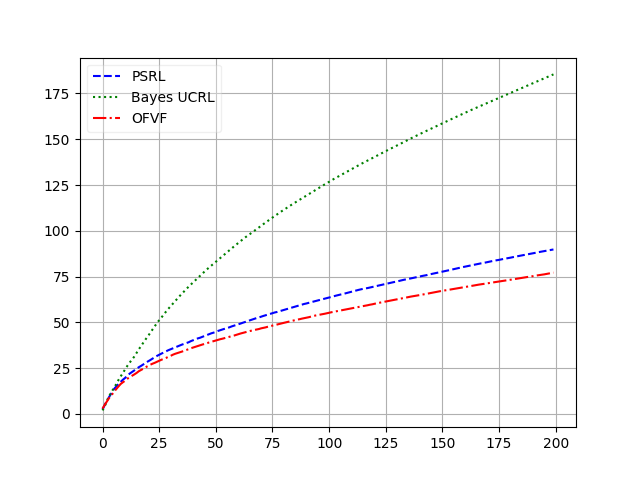
\includegraphics[width=\linewidth]{figures/SimpleProblem_PSRL_BayesUCRL_OFVF.png}
	\end{minipage}%
	\begin{minipage}[c]{.45\columnwidth}
		\centering
		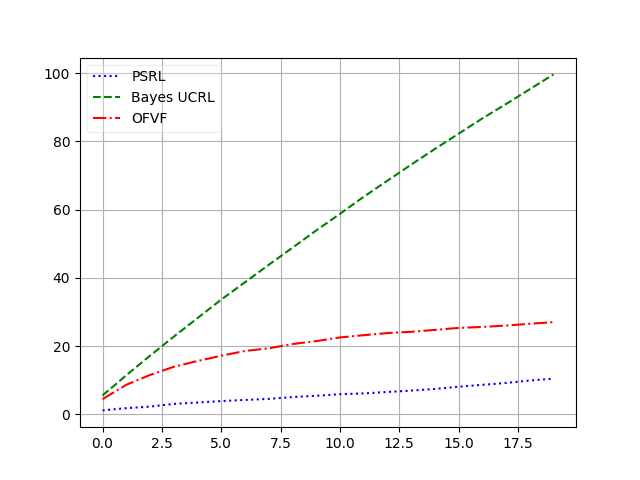
\includegraphics[width=\linewidth]{figures/RiverSwim_RSVF_BAYESUCB_PSRL.png}
	\end{minipage}%
	\caption{Cumulative regrets of PSRL and Bayes UCRL: left) above described simple problem, right) RiverSwim Problem described in \citep{Osband2013}}
	\label{fig:dirichlet_result}
\end{figure}

\section{Conclusion}

Summarize the paper

% Acknowledgements should only appear in the accepted version.
\section*{Acknowledgements}

\textbf{Do not} include acknowledgements in the initial version of
the paper submitted for blind review.

If a paper is accepted, the final camera-ready version can (and
probably should) include acknowledgements. In this case, please
place such acknowledgements in an unnumbered section at the
end of the paper. Typically, this will include thanks to reviewers
who gave useful comments, to colleagues who contributed to the ideas,
and to funding agencies and corporate sponsors that provided financial
support.

% In the unusual situation where you want a paper to appear in the
% references without citing it in the main text, use \nocite
\nocite{langley00}

\bibliography{ofvf}
\bibliographystyle{icml2018}


%%%%%%%%%%%%%%%%%%%%%%%%%%%%%%%%%%%%%%%%%%%%%%%%%%%%%%%%%%%%%%%%%%%%%%%%%%%%%%%
%%%%%%%%%%%%%%%%%%%%%%%%%%%%%%%%%%%%%%%%%%%%%%%%%%%%%%%%%%%%%%%%%%%%%%%%%%%%%%%
% DELETE THIS PART. DO NOT PLACE CONTENT AFTER THE REFERENCES!
%%%%%%%%%%%%%%%%%%%%%%%%%%%%%%%%%%%%%%%%%%%%%%%%%%%%%%%%%%%%%%%%%%%%%%%%%%%%%%%
%%%%%%%%%%%%%%%%%%%%%%%%%%%%%%%%%%%%%%%%%%%%%%%%%%%%%%%%%%%%%%%%%%%%%%%%%%%%%%%
\appendix
\section{Do \emph{not} have an appendix here}

\textbf{\emph{Do not put content after the references.}}
%
Put anything that you might normally include after the references in a separate
supplementary file.

We recommend that you build supplementary material in a separate document.
If you must create one PDF and cut it up, please be careful to use a tool that
doesn't alter the margins, and that doesn't aggressively rewrite the PDF file.
pdftk usually works fine. 

\textbf{Please do not use Apple's preview to cut off supplementary material.} In
previous years it has altered margins, and created headaches at the camera-ready
stage. 
%%%%%%%%%%%%%%%%%%%%%%%%%%%%%%%%%%%%%%%%%%%%%%%%%%%%%%%%%%%%%%%%%%%%%%%%%%%%%%%
%%%%%%%%%%%%%%%%%%%%%%%%%%%%%%%%%%%%%%%%%%%%%%%%%%%%%%%%%%%%%%%%%%%%%%%%%%%%%%%


\end{document}


% This document was modified from the file originally made available by
% Pat Langley and Andrea Danyluk for ICML-2K. This version was created
% by Iain Murray in 2018. It was modified from a version from Dan Roy in
% 2017, which was based on a version from Lise Getoor and Tobias
% Scheffer, which was slightly modified from the 2010 version by
% Thorsten Joachims & Johannes Fuernkranz, slightly modified from the
% 2009 version by Kiri Wagstaff and Sam Roweis's 2008 version, which is
% slightly modified from Prasad Tadepalli's 2007 version which is a
% lightly changed version of the previous year's version by Andrew
% Moore, which was in turn edited from those of Kristian Kersting and
% Codrina Lauth. Alex Smola contributed to the algorithmic style files.
